\chapter{Memisahkan Campuran}\label{ch:g3:separating-mixtures}

Sehabis badai, genangan di jalan berwarna cokelat: air hujan bercampur
tanah, pasir, dan serpihan daun. Padahal air yang keluar dari keran
dapur jernih, dan air itu pun dulunya air hujan, sebelum mengalir ke
sungai. Bagaimana air berlumpur dapat dibuat bersih lagi? Benda-benda
yang sudah \omterm{def:g2:mixing-and-dissolving:mix}{dicampur} dapat dipisahkan lagi. Bab ini menunjukkan caranya,
satu metode demi satu metode.

\begin{recall}
\omterm{def:g2:mixing-and-dissolving:mix}{Mencampur} berarti menyatukan benda-benda yang berbeda. Padatan seperti
gula atau garam \omterm{def:g2:mixing-and-dissolving:dissolve}{larut} dalam air: padatan itu hilang dari pandangan, dan
cairan jernih yang terbentuk adalah larutan. Padatan yang \omterm{def:g2:mixing-and-dissolving:dissolve}{larut} masih
ada: ketika airnya mengering, padatan itu tertinggal. Pasir dan tanah
tidak \omterm{def:g2:mixing-and-dissolving:dissolve}{larut} (\cref{ch:g2:mixing-and-dissolving}).
\end{recall}

\section{Memilah dengan tangan dan mengayak}

Jika bagian-bagian sebuah campuran cukup besar untuk dilihat dan
dipungut, cara paling sederhana untuk memisahkannya adalah dengan
tangan: kismis dapat dipungut satu per satu dari muesli. Jika bagiannya
terlalu banyak, ayakanlah yang memilahkannya untuk kita.

\begin{definition}[Pengayakan]\label{def:g3:separating-mixtures:sieve}
Yang disebut \emph{pengayakan}\index{pengayakan} adalah memisahkan
bagian-bagian sebuah campuran menurut ukurannya, dengan ayakan: jaring
atau pelat yang penuh lubang. Bagian yang kecil jatuh melewati lubang;
bagian yang besar tertahan di ayakan.
\end{definition}

\begin{example}[Kerikil dan pasir]\label{ex:g3:separating-mixtures:gravel}
Seorang tukang bangunan mengguncang campuran kerikil dan pasir di atas
ayakan. Pasir halus jatuh menembus ayakan dan membentuk tumpukan di
bawahnya; kerikil tertahan di atas jaring.
\end{example}

\begin{omfigure}
\begin{tikzpicture}[font=\small]
  % the sieve: a mesh bowl
  \fill[pattern=crosshatch, pattern color=black!45] (-1.6,2.6) arc[start angle=180,
    end angle=360, x radius=1.6, y radius=0.7] -- cycle;
  \draw[black!70, line width=0.8pt] (-1.6,2.6) arc[start angle=180, end angle=360,
    x radius=1.6, y radius=0.7];
  \draw[black!70, line width=0.8pt] (-1.75,2.6) -- (1.75,2.6);
  \draw[black!70, line width=1.4pt] (1.75,2.6) -- (3.0,2.85);
  % gravel kept in the sieve
  \foreach \x/\y/\r in {-0.9/2.25/0.17,-0.45/2.12/0.2,0.05/2.08/0.18,0.5/2.13/0.21,
                        0.95/2.28/0.16,-0.2/2.42/0.15,0.3/2.43/0.17}
    \fill[black!45, draw=black!65] (\x,\y) circle (\r);
  % sand falling
  \foreach \x/\y in {-0.4/1.6,0.1/1.4,0.4/1.7,-0.15/1.15,0.25/1.0,-0.5/0.95,0.0/0.75}
    \fill[orange!60!brown] (\x,\y) circle (0.05);
  % the heap of sand in a bowl
  \fill[orange!45!brown!70] (-1.0,0.12) .. controls (-0.5,0.55) and (0.5,0.55)
    .. (1.0,0.12) -- cycle;
  \draw[black!70, line width=0.8pt] (-1.5,0.5) .. controls (-1.3,0) and (1.3,0)
    .. (1.5,0.5);
  \node[anchor=west] at (2.0,2.2) {kerikil tertahan di ayakan};
  \node[anchor=west] at (2.0,1.25) {pasir jatuh melewati lubang};
  \node[anchor=west] at (2.0,0.3) {tumpukan pasir};
\end{tikzpicture}

{\small Mengayak campuran kerikil dan pasir: bagian-bagiannya dipilah
menurut ukuran.}
\end{omfigure}

\begin{omfigure}
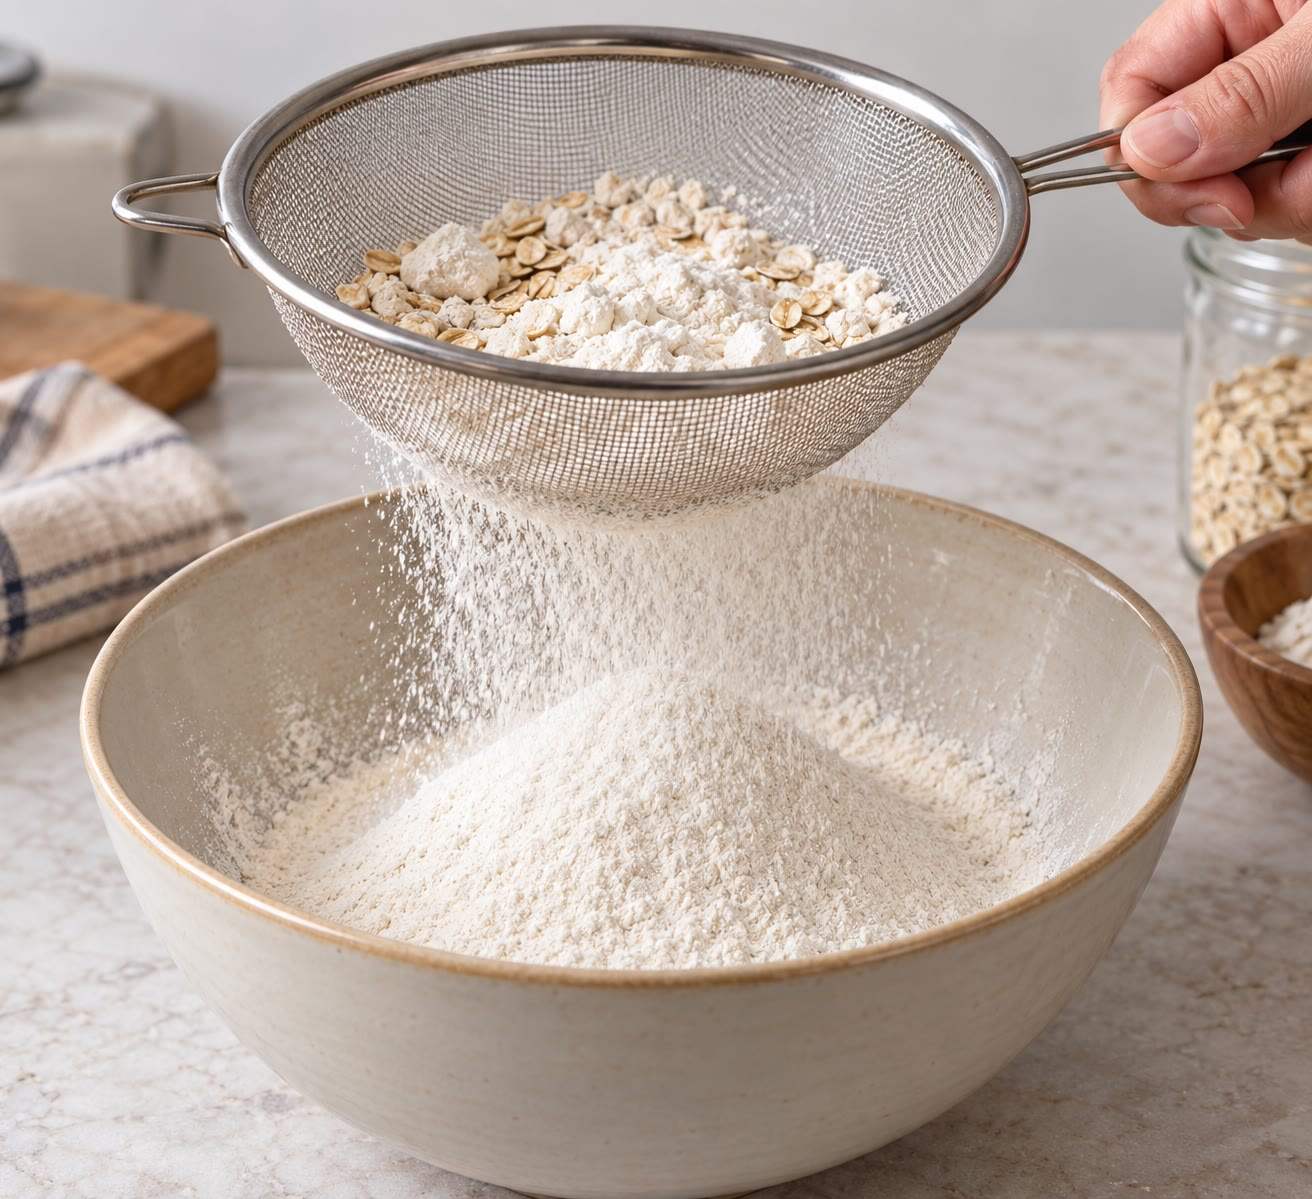
\includegraphics[width=0.55\linewidth]{images/book1/ai/g3-kitchen-sieve.jpg}

{\small Ayakan dapur: tepung yang halus lolos, gumpalannya tertahan.}
\end{omfigure}

\section{Mengendapkan dan dekantasi}

\begin{definition}[Pengendapan dan dekantasi]\label{def:g3:separating-mixtures:decant}
Campuran air dengan padatan yang tidak \omterm{def:g2:mixing-and-dissolving:dissolve}{larut} dapat dibiarkan diam:
padatan itu perlahan-lahan turun ke dasar. Peristiwa ini disebut
\emph{pengendapan}\index{pengendapan}. Setelah padatan mengendap, air
jernih di atasnya dapat dituang perlahan ke wadah lain, sementara
padatannya tertinggal: inilah \emph{dekantasi}\index{dekantasi}.
\end{definition}

\begin{omfigure}
\begin{tikzpicture}[font=\small]
  % 1: stirred, cloudy
  \pic at (0,0) {beaker={0.7}{brown!28}};
  \foreach \x/\y in {-0.5/0.3,-0.2/0.6,0.3/0.4,0.5/0.9,-0.4/1.0,0.1/1.2,0.4/0.15,
                     -0.1/0.25,0.2/0.8,-0.55/0.7}
    \fill[brown!60] (\x,\y) circle (0.03);
  \node[anchor=north, align=center] at (0,-0.15) {diaduk:\\ keruh};
  \draw[->, thick, omProp] (1.1,1.0) -- (2.4,1.0);
  % 2: settled
  \pic at (3.5,0) {beaker={0.7}{omWater!80}};
  \fill[brown!60] (2.7,0) rectangle (4.3,0.25);
  \draw[omGlass, line width=0.7pt] (2.7,0.25) -- (2.7,0) -- (4.3,0) -- (4.3,0.25);
  \node[anchor=north, align=center] at (3.5,-0.15) {dibiarkan diam:\\ tanah mengendap};
  \draw[->, thick, omProp] (4.6,1.0) -- (5.9,1.0);
  % 3: decanted
  \pic at (7.0,0) {beaker={0.1}{omWater!80}};
  \fill[brown!60] (6.2,0) rectangle (7.8,0.25);
  \draw[omGlass, line width=0.7pt] (6.2,0.25) -- (6.2,0) -- (7.8,0) -- (7.8,0.25);
  \pic at (9.2,0) {beaker={0.58}{omWater!80}};
  \node[anchor=north, align=center] at (8.1,-0.15) {dituang: air jernih\\ di kanan, tanah tertinggal};
\end{tikzpicture}

{\small \omterm{def:g3:separating-mixtures:decant}{Pengendapan}, lalu \omterm{def:g3:separating-mixtures:decant}{dekantasi} campuran tanah dan air.}
\end{omfigure}

\begin{remark}[Mengendap butuh waktu]\label{rem:g3:separating-mixtures:time}
Butiran yang besar dan berat mengendap dalam beberapa menit; lempung
yang sangat halus dapat butuh sehari atau lebih, dan selama itu airnya
tetap agak keruh. \omterm{def:g3:separating-mixtures:decant}{Dekantasi} tidak pernah membuang semua butiran:
sedikit kekeruhan ikut tertuang bersama air.
\end{remark}

\section{Menyaring}

\begin{definition}[Penyaringan dan filtrat]\label{def:g3:separating-mixtures:filter}
Yang disebut \emph{penyaringan}\index{penyaringan} adalah menuang
campuran melalui saringan: selembar kertas, sehelai kain, atau selapis
pasir yang lubangnya terlalu kecil untuk dilewati bagian-bagian padat.
Padatannya tertahan di saringan; cairan jernih yang lolos disebut
\emph{filtrat}\index{filtrat}.
\end{definition}

\begin{omfigure}
\begin{tikzpicture}[font=\small, scale=1.4]
  \pic[transform shape] at (0,0) {beaker={0.35}{omWater!80}};
  \pic[transform shape] at (0,1.4) {funnel={brown!55}};
  % muddy water waiting in the paper cone, above the soil
  \fill[brown!25] (-0.411,2.45) -- (0.411,2.45) -- (0.722,2.8) -- (-0.722,2.8) -- cycle;
  % drops of filtrate
  \foreach \y in {1.15,0.95} \fill[omDef!50] (0,\y) circle (0.04);
  \draw[<-, omProp, thick] (0.75,2.6) -- (2.0,2.9) node[right, text=black]
    {kertas saring di dalam corong};
  \draw[<-, omProp, thick] (0.25,2.15) -- (2.0,2.2) node[right, text=black]
    {tanah tertahan di kertas};
  \draw[<-, omProp, thick] (0.85,0.4) -- (2.0,0.6) node[right, text=black]
    {filtrat: air jernih};
\end{tikzpicture}

{\small Menyaring air berlumpur dengan kertas saring.}
\end{omfigure}

\begin{inthelab}[Menyaring air berlumpur]
Guru melipat selembar kertas saring yang bundar menjadi kerucut dan
memasangnya di dalam corong kaca di atas sebuah gelas kimia. Air
berlumpur dituang ke dalam kerucut, sedikit demi sedikit, tidak pernah
melewati tepi kertas. Air jernih menetes ke dalam gelas kimia; tanah
membentuk lapisan cokelat di atas kertas. Jika \omterm{def:g3:separating-mixtures:filter}{filtratnya} keruh,
berarti kertasnya sobek atau airnya meluap melewati tepinya.
\end{inthelab}

\begin{proposition}[Saringan tidak menahan zat yang larut]\label{prop:g3:separating-mixtures:dissolved}
Saringan menahan bagian-bagian padat yang tidak \omterm{def:g2:mixing-and-dissolving:dissolve}{larut}. Saringan tidak
menahan apa yang \omterm{def:g2:mixing-and-dissolving:dissolve}{larut}: air asin yang dituang melalui saringan keluar
sama asinnya, dan teh manis sama manisnya.
\end{proposition}

\begin{omfigure}
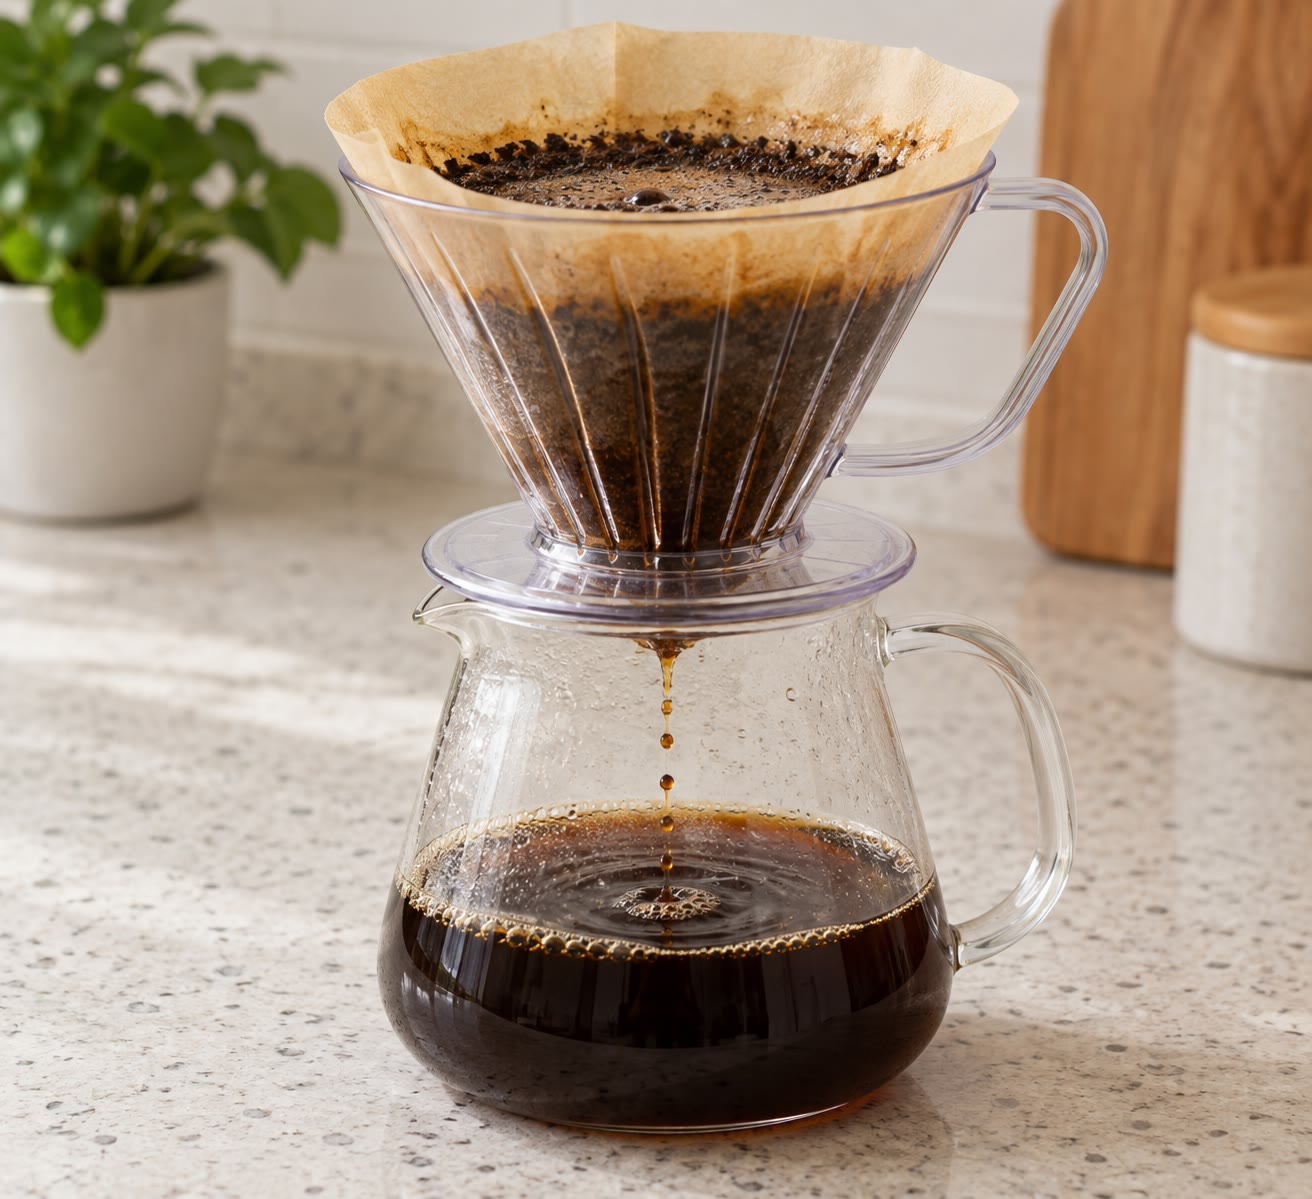
\includegraphics[width=0.5\linewidth]{images/book1/ai/g3-coffee-filter.jpg}

{\small Membuat kopi berarti menyaring: ampasnya tertahan di kertas,
kopinya adalah \omterm{def:g3:separating-mixtures:filter}{filtrat}.}
\end{omfigure}

\section{Menguapkan airnya}

\begin{definition}[Penguapan]\label{def:g3:separating-mixtures:evaporate}
Untuk mendapatkan kembali padatan yang \omterm{def:g2:mixing-and-dissolving:dissolve}{larut} dalam air, airnya
dibiarkan mengering, di bawah matahari atau di atas api kecil: inilah
\emph{penguapan}\index{penguapan}. Airnya pergi ke udara; padatannya
tertinggal di cawan.
\end{definition}

\begin{example}[Garam dari air asin]\label{ex:g3:separating-mixtures:salt}
Sedikit air asin dituang ke cawan dangkal dan dibiarkan di ambang
jendela yang terkena sinar matahari. Beberapa hari kemudian airnya
habis, yang tersisa hanya kerak putih garam: garam yang tadinya \omterm{def:g2:mixing-and-dissolving:dissolve}{larut}.
\end{example}

\begin{omfigure}
\begin{tikzpicture}[font=\small, scale=1.4]
  \pic[transform shape] at (0,0) {hotplate};
  \pic[transform shape] at (0,0) {evapdish={omWater!80}};
  \node[anchor=north, align=center] at (0,-0.6) {air asin,\\ dipanaskan pelan};
  \draw[->, thick, omProp] (1.5,0.3) -- (3.0,0.3) node[midway, above, text=black]
    {kemudian};
  \pic[transform shape] at (4.5,0) {hotplate};
  \pic[transform shape] at (4.5,0) {evapdish={white!85!black}};
  \foreach \x in {-0.45,-0.25,-0.05,0.15,0.35}
    \fill[white, draw=black!45, line width=0.2pt] (4.5+\x,0.12) rectangle ++(0.09,0.06);
  \node[anchor=north, align=center] at (4.5,-0.6) {airnya habis:\\ kristal garam};
  \foreach \x in {-0.3,0,0.3} \draw[->, black!45, decorate,
    decoration={snake, amplitude=0.6pt, segment length=4pt}] (\x,0.7) -- (\x,1.4);
  \node[anchor=south] at (0,1.4) {air pergi ke udara};
\end{tikzpicture}

{\small \omterm{def:g3:separating-mixtures:evaporate}{Penguapan} di laboratorium: guru menghangatkan cawan perlahan di
atas pelat pemanas. Garamnya tertinggal di cawan.}
\end{omfigure}

\section{Metode mana untuk campuran mana?}

\begin{method}[Memilih cara pemisahan]\label{met:g3:separating-mixtures:choose}
Untuk memisahkan sebuah campuran, tanyakan:
\begin{enumerate}
  \item Apakah bagian-bagiannya besar dan berbeda ukurannya? Pilahlah
        dengan tangan, atau ayaklah.
  \item Adakah padatan yang tidak \omterm{def:g2:mixing-and-dissolving:dissolve}{larut} di dalam cairan? Biarkan
        mengendap lalu lakukan \omterm{def:g3:separating-mixtures:decant}{dekantasi}, atau saringlah agar airnya
        lebih jernih.
  \item Adakah padatan yang \omterm{def:g2:mixing-and-dissolving:dissolve}{larut} di dalam cairan? \omterm{def:g3:separating-mixtures:evaporate}{Uapkan} cairannya:
        padatannya tertinggal.
\end{enumerate}
Sering kali diperlukan beberapa langkah, satu sesudah yang lain.
\end{method}

\begin{example}[Pasir, garam, dan air]\label{ex:g3:separating-mixtures:three}
Sebuah stoples berisi air yang \omterm{def:g2:mixing-and-dissolving:mix}{dicampur} pasir dan garam. Garamnya \omterm{def:g2:mixing-and-dissolving:dissolve}{larut};
pasirnya tidak.
\begin{enumerate}
  \item Saring: pasirnya tertahan di kertas.
  \item \omterm{def:g3:separating-mixtures:filter}{Filtratnya} jernih, tetapi berupa air asin. \omterm{def:g3:separating-mixtures:evaporate}{Uapkan} \omterm{def:g3:separating-mixtures:filter}{filtrat} itu:
        garamnya tertinggal di cawan.
\end{enumerate}
Dua metode, satu sesudah yang lain, mengembalikan pasir dan garamnya.
\end{example}

\begin{example}[Air bersih dari sungai]\label{ex:g3:separating-mixtures:plant}
Instalasi pengolahan air membuat air sungai layak minum dalam beberapa
langkah:
\begin{enumerate}
  \item air sungai melewati saringan kasar, yaitu jeruji besar yang
        menahan ranting, daun, dan plastik: semacam \omterm{def:g3:separating-mixtures:sieve}{pengayakan};
  \item air itu didiamkan di bak-bak besar tempat lumpur mengendap ke
        dasar;
  \item air disaring melalui lapisan pasir yang tebal, yang menahan
        butiran paling halus;
  \item sedikit sekali bahan pembunuh kuman ditambahkan, supaya air
        tetap aman di dalam pipa.
\end{enumerate}
\end{example}

\begin{omfigure}
\begin{tikzpicture}[font=\small, node distance=0.45cm,
    box/.style={draw=omDef, fill=omDef!6, rounded corners=2pt, align=center,
      minimum height=1.15cm, text width=2.0cm}]
  \node[box] (r) {air\\ sungai};
  \node[box, right=of r] (s) {jeruji\\ (pengayakan)};
  \node[box, right=of s] (t) {bak\\ pengendap};
  \node[box, right=of t] (f) {saringan\\ pasir};
  \node[box, right=of f] (g) {pembasmian\\ kuman};
  \foreach \a/\b in {r/s,s/t,t/f,f/g} \draw[->, thick, omProp] (\a) -- (\b);
  \node[below=0.15cm of s, font=\footnotesize, align=center] {ranting,\\ plastik};
  \node[below=0.15cm of t, font=\footnotesize, align=center] {lumpur};
  \node[below=0.15cm of f, font=\footnotesize, align=center] {butiran halus};
  \draw[->, thick, omProp] (g.south) -- ++(0,-0.8) node[below] {ke keran};
\end{tikzpicture}

{\small Langkah-langkah instalasi pengolahan air. Di bawah setiap
langkah: apa yang dibuangnya.}
\end{omfigure}

\begin{omfigure}
\begin{minipage}[t]{0.48\linewidth}\centering
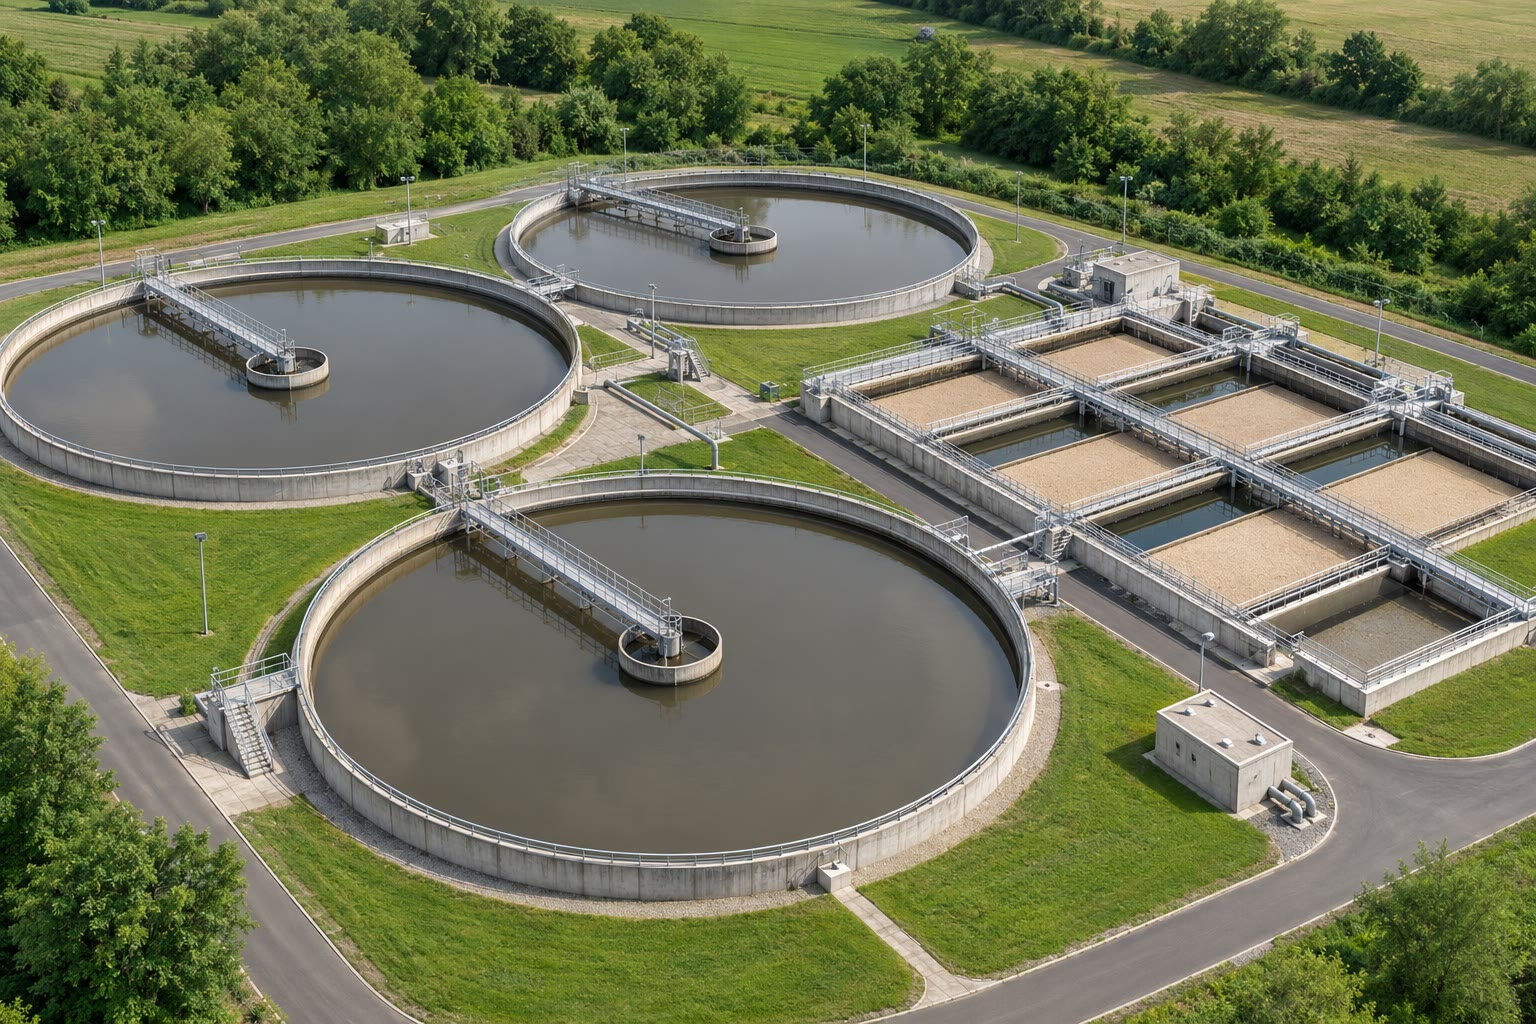
\includegraphics[width=\linewidth,height=4.6cm,keepaspectratio]{images/book1/ai/g3-settling-tanks.jpg}

{\small Bak pengendap di instalasi pengolahan air.}
\end{minipage}\hfill
\begin{minipage}[t]{0.48\linewidth}\centering
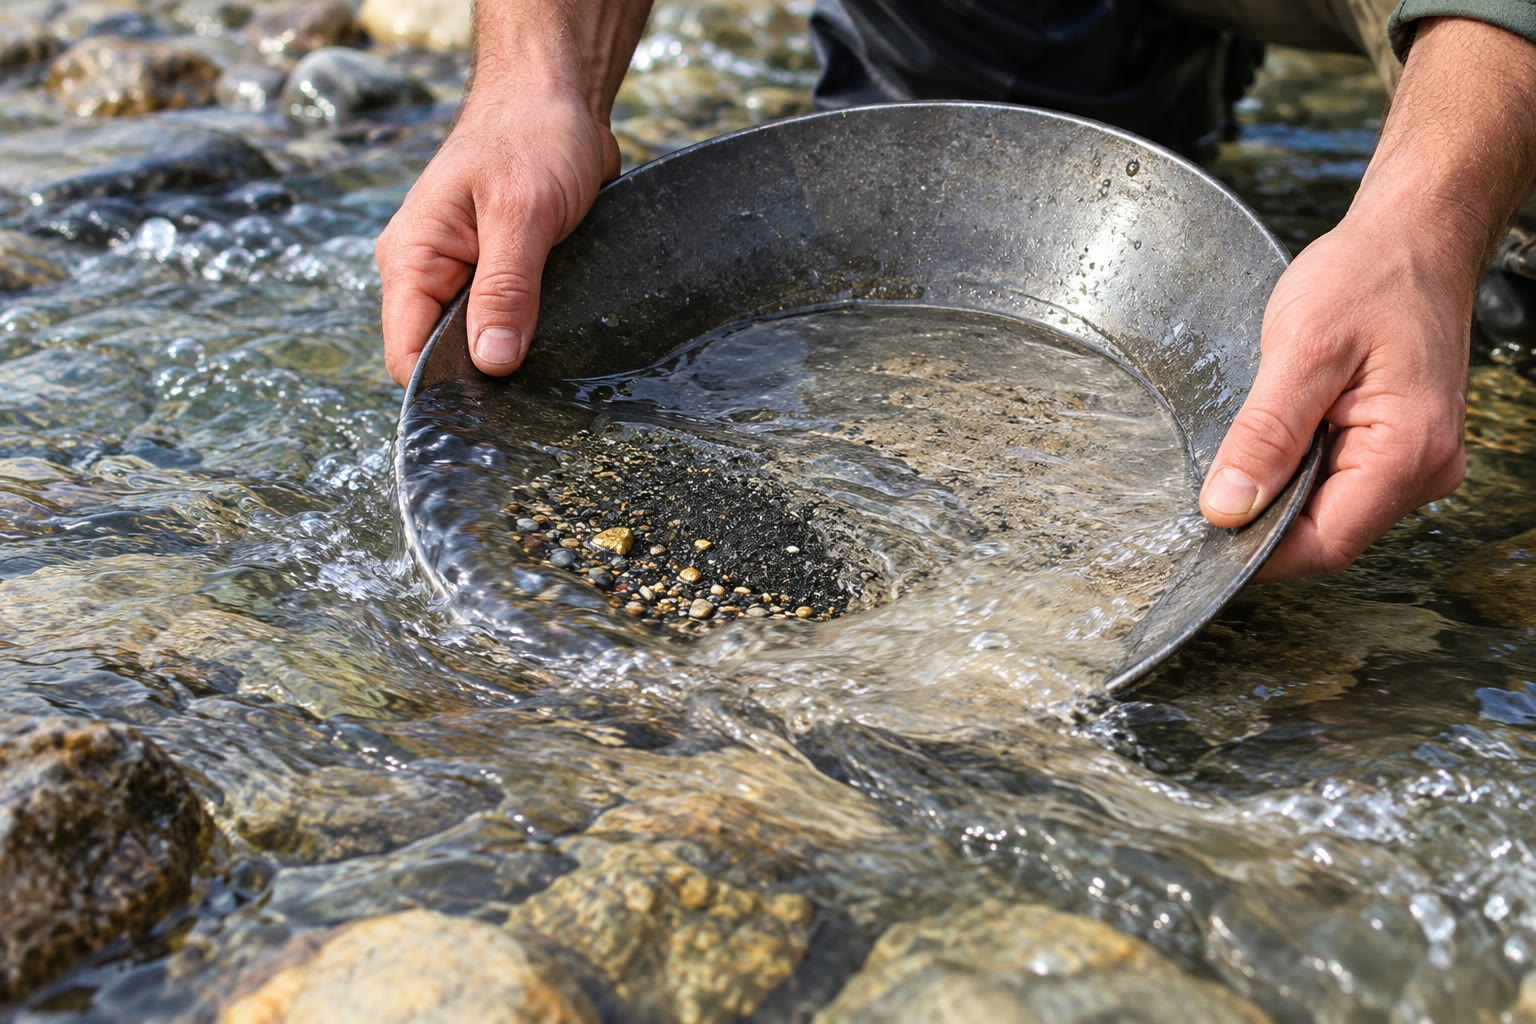
\includegraphics[width=\linewidth,height=4.6cm,keepaspectratio]{images/book1/ai/g3-gold-panning.jpg}

{\small Mendulang emas: air sungai menghanyutkan pasir yang ringan;
butiran yang berat tertinggal di dulang.}
\end{minipage}
\end{omfigure}

\begin{remark}[Jernih belum tentu bersih]\label{rem:g3:separating-mixtures:clean}
Air yang sudah disaring dapat tampak sangat jernih tetapi masih
mengandung zat yang \omterm{def:g2:mixing-and-dissolving:dissolve}{larut}, juga kuman yang jauh terlalu kecil untuk
dilihat. Karena itulah tidak seorang pun meminum air dari genangan atau
dari sungai kecil, sekalipun sudah disaring.
\end{remark}

\section{Latihan}

\begin{exercise}[$\star$]\label{exo:g3:separating-mixtures:1}
Metode apa yang akan kamu pakai untuk memisahkan kacang polong dari
butiran beras?
\end{exercise}

\begin{exercise}[$\star$]\label{exo:g3:separating-mixtures:2}
Segelas air berlumpur dibiarkan di atas meja selama satu jam. Apa yang
terjadi pada tanahnya? Disebut apakah peristiwa ini?
\end{exercise}

\begin{exercise}[$\star$]\label{exo:g3:separating-mixtures:3}
Apa itu \omterm{def:g3:separating-mixtures:filter}{filtrat}? Sebutkan \omterm{def:g3:separating-mixtures:filter}{filtratnya} ketika orang membuat kopi.
\end{exercise}

\begin{exercise}[$\star$]\label{exo:g3:separating-mixtures:4}
Air asin dituang melalui kertas saring. Apakah \omterm{def:g3:separating-mixtures:filter}{filtratnya} asin?
Jelaskan.
\end{exercise}

\begin{exercise}[$\star$]\label{exo:g3:separating-mixtures:5}
Bagaimana gula dapat diperoleh kembali dari segelas air gula?
\end{exercise}

\begin{exercise}[$\star$]\label{exo:g3:separating-mixtures:6}
Lihatlah gambar ayakan. Bagian mana yang tertahan di ayakan? Mengapa
bagian yang lain jatuh melewatinya?
\end{exercise}

\begin{exercise}[$\star$]\label{exo:g3:separating-mixtures:7}
Pasangkan setiap campuran dengan sebuah metode --- \omterm{def:g3:separating-mixtures:sieve}{pengayakan},
\omterm{def:g3:separating-mixtures:filter}{penyaringan}, atau \omterm{def:g3:separating-mixtures:evaporate}{penguapan}: (a) pasir dan kerikil; (b) serbuk kapur
tulis dalam air; (c) garam dalam air.
\end{exercise}

\begin{exercise}[$\star$]\label{exo:g3:separating-mixtures:8}
Lihatlah gambar instalasi pengolahan air. Berapa langkah yang dilalui
air? Langkah mana yang membuang lumpur?
\end{exercise}

\begin{exercise}[$\star$]\label{exo:g3:separating-mixtures:9}
Urutkan langkah-langkah berikut untuk mendapatkan kembali pasir dan
garam dari stoples berisi pasir, garam, dan air: \omterm{def:g3:separating-mixtures:evaporate}{uapkan} \omterm{def:g3:separating-mixtures:filter}{filtratnya};
saring; ambil pasir dari kertas saring.
\end{exercise}

\begin{exercise}[$\star\star$]\label{exo:g3:separating-mixtures:10}
Dapatkah saringan membuat air laut layak minum? Jelaskan mengapa tidak.
\end{exercise}

\begin{exercise}[$\star\star$]\label{exo:g3:separating-mixtures:11}
Daun teh tertinggal di dalam teko yang penuh teh. Sebutkan dua metode
dari bab ini yang memisahkan teh dari daunnya.
\end{exercise}
